
\chapter{Controles}
É possível aumentar e baixar a velocidade usando o botão "up" e "down" do teclado. O avião também pode realizar curvas. 
Isso pode ser feito usando as setas do teclado; quando a seta é solta, o avião volta para o voo nivelado mantendo a proa constante. Enquanto a tecla da direita é pressionada o avião aumenta o ângulo de proa em uma razão constante, enquanto a tecla esquerda é pressionada a proa diminui também em razão constante.

A proa pode variar de 0 graus a 359. Ocorre underflow quando o valor fica menor que zero e overflow quando fica maior que 359.

\begin{verbatim}
    
357        358         359   <-- -1 -- +1 -->  0        1        2
                        
\end{verbatim}

Também é possível usar o mouse; nesse caso, com o cursor na posição central da janela, o voo é mantido nivelado. A distância para a direita ou esquerda determina o quanto a aeronave inclinará para o lado escolhido, permitindo fazer uma curva mais fechada ou aberta. O avião só voltará para o voo nivelado caso o cursor seja recolocado na posição central.

Apenas a coordenada X do mouse importa; a coordenada Y é descartada.

Sendo:

\begin{itemize}
\item W: largura da tela;
\item R\_max: Razão máxima de mudança do ângulo da proa;
\item R: Razão atual de mudança do ângulo da proa;
\item delta: explicado anteriormente;
\item heading: proa atual.
\end{itemize}


A proa atual é calculada por
\texttt{heading += R * delta}

Para se achar o \texttt{R} usa-se a posição x do cursor dentro da tela.

\begin{figure}[h]
    \centering
    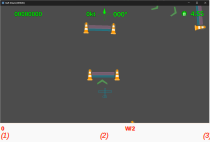
\includegraphics[width=\textwidth]{mouse-x.png}
\end{figure}

\begin{itemize}
\item \textbf{(1)} = cursor no canto esquerdo da janela: \texttt{R = -R\_max}
\item \textbf{(2)} = cursor no meio da janela: \texttt{R = 0}
\item \textbf{(3)} = cursor no canto direito da janela: \texttt{R = R\_max}
\end{itemize}

Para valores entre '1 e 2' e '2 e 3' é feita interpolação linear.

\section*{Gameplay}
Como na corrida real, o avião deve passar pelos chamados "Air gates", que são duas colunas (pylon na Red Bull Air Race real) pelas quais a aeronave deve passar no meio, exigindo destreza e timing, já que nenhuma parte do avião pode tocar nas colunas. Na competição real, essas colunas são cones de nylon inflados com ar, como balões que não causam danos à aeronave em caso de colisão, apenas o material se rasga, indicando que o avião não passou corretamente.

\begin{figure}[h]
    \centering
    \includegraphics[width=0.8\textwidth]{red-bull-2.jpg}
\end{figure}

\section*{Air Gate}
Existem dois tipos de Air gates: o largo e o estreito.

\subsection*{Largo}
No largo, o avião deve passar sem tocar em nenhuma parte nas colunas. Caso toque, são descontados 100 pontos. Existe um sentido correto para passar; caso passe no sentido errado, são perdidos 500 pontos.

\subsection*{Estreito}
No Air gate estreito, as regras anteriores também valem, mas uma dificuldade extra é adicionada. Quando estiver passando, o avião deve estar com as asas inclinadas, mais precisamente com \texttt{abs(R) >= R\_max / 2}. O significado de \texttt{R} e \texttt{R\_max} foi explicado anteriormente. 
Caso esta regra seja descumprida, são descontados 50 pontos. O desconto é cumulativo, então, caso o avião passe em voo nivelado e atinja um dos cones, são perdidos 150 pontos.

\section*{Power up/down}
O jogo dura 5 minutos, mas aparecem em posições aleatórias do mapa "power-ups" de tempos que dão 30 segundos extras caso o avião passe por cima de um. 
Este possui a cor verde. Caso esteja na cor vermelha é descontado 1 minuto. Ambos os power-ups desaparecem ao serem passados.

\section*{ExtraHealth}
Existe também um power up que, caso o avião atravesse-o, é dada uma vida extra.

\section*{Caminho}
O avião deve seguir a ordem de "airgates" mantendo-se dentro de um caminho pre-estabelecido. A cada delta, a distância do avião ao caminho é calculada. A partir de um limiar, o jogador começa a perder ponto em uma razão proporcional à distância do caminho. Caso ele fique muito longe, em poucos segundos seu escore chega a zero e ele perde.

\section*{Término do jogo}
O jogo termina se uma ou mais destas condições ocorrerem:
\begin{enumerate}
    \item O tempo chegar em zero;
    \item Os pontos do jogador ficarem iguais a zero ou negativos.
\end{enumerate}
